\documentclass[12pt]{article}
\usepackage{preamble}

\pagestyle{fancy}
\fancyhead[LO,LE]{Математический анализ}
\fancyhead[CO,CE]{14.02.2024}
\fancyhead[RO,RE]{Лекции Далевской О. П.}


\begin{document}
    \section{1.4. Приложения определенного интеграла}
    \hypertarget{integralapplications}{}

    \section{1.4.1. Площади}

    1* \Mem \hypertarget{integralareadpsk}{Значение интеграла} - площадь фигуры под графиком

    \begin{center}
        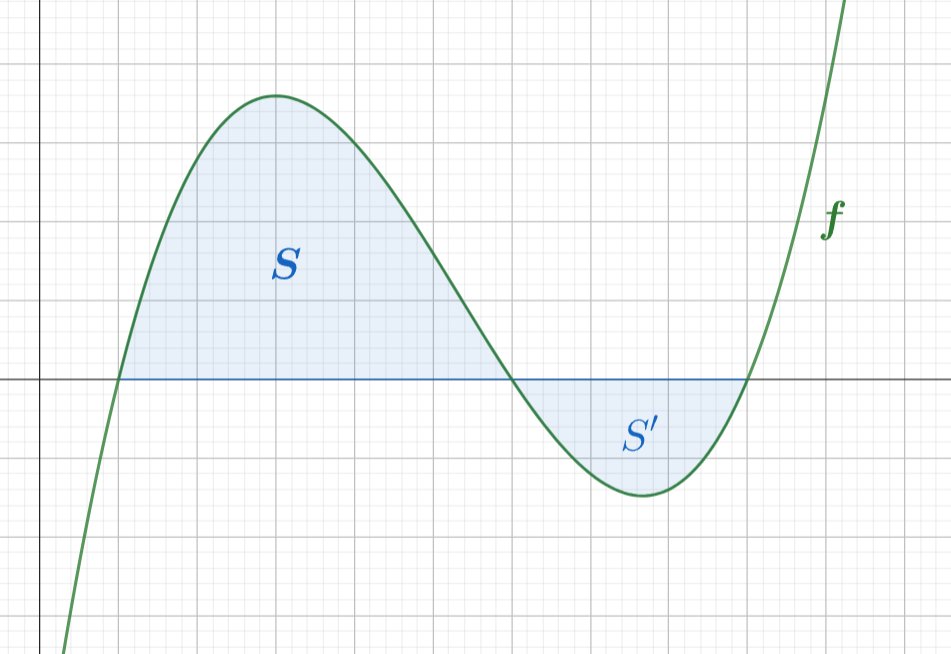
\includegraphics[height=6cm]{calculus/images/calculus_2024_02_14_1}
    \end{center}

    \underline{Геом. смысл}. $S = \int_a^b f(x) dx \quad\quad S^\prime = -\int_b^c f(x)dx$

    \mediumvspace

    2*

    \begin{center}
        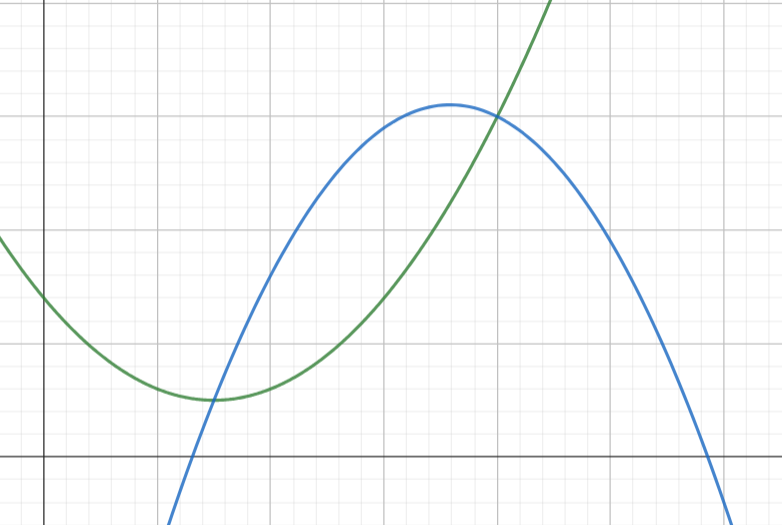
\includegraphics[height=6cm]{calculus/images/calculus_2024_02_14_3}
    \end{center}

    Площадь фигуры, окруженной графиками функций $S = \int_a^b |f(x) - g(x)| dx$, $a, b$ - абсциссы точек пересечения

    \Nota Симметрия

    Если $f(x)$ - четная функция, то $\int_{-a}^a f(x) dx = 2 \int_0^a f(x)dx$

    Если $f(x)$ - нечетная функция, то $\int_{-a}^a f(x) dx = 0$

    \section{1.4.2. Площадь в ПСК}

    \hypertarget{integralareapsk}{В ДПСК мы производили дробление фигуры на элементарные прямоугольники.} Сделаем подобное в ПСК для $\rho(\varphi)$:

    1) Дробление $[\alpha;\beta]$ на угловые сектора $[\varphi_{i - 1};\varphi_i]$

    $\Delta \varphi_i$ - угол сектора

    2) Выбор средней точки $\psi_i \in [\varphi_{i - 1};\varphi_i]$, площадь сектора $S_i = \frac{1}{2} \Delta \varphi_i \rho^2(\psi_i)$

    3) Интегральная сумма $\sigma_n = \frac{1}{2} \sum_{i=1}^n \rho^2 (\varphi_i) \Delta \varphi_i$

    4) Предел $\lim_{n \to \infty} \frac{1}{2} \sum_{i=1}^n \rho^2 (\varphi_i) \Delta \varphi_i = \frac{1}{2} \int_\alpha^\beta \rho^2(\varphi) d\varphi$

    \Ex Кардиоида:

    $\rho = 1 + \cos\varphi$

    $S = \frac{1}{2}\int^{\pi}_{-\pi} \rho^2 (\varphi) \Delta \varphi = \int_0^\pi \rho^2 (\varphi) \Delta \varphi =
    \int_0^\pi (1 + \cos\varphi)^2 \Delta \varphi = \int_0^\pi (1 + 2\cos\varphi + \cos^2\varphi) \Delta \varphi =
    \varphi \Big|_0^\pi + \int_0^\pi \frac{1 + \cos2\varphi}{2} \Delta \varphi = \pi + \frac{1}{2}\pi = \frac{3}{2}\pi$

    \Nota Если фигура задана параметрическими уравнениями:

    $\begin{cases}x = x(t) \\ y = y(t)\end{cases} \quad \alpha \leq t \leq \beta$

    То площадь будет равна $S = \int_a^b y(x)dx = \int^\beta_\alpha y(t)x^\prime(t)dt$

    \section{1.4.3. Длина кривой дуги}

    \hypertarget{lengthofarc}{Пусть дуга $AB$ задана уравнением $y = f(x) \quad x \in [a;b]$}

    \begin{enumerate}
        \item Производим дробление дуги на элементарные дуги точками $A = M_0 < M_1 < \dots < B = M_n$

        Здесь порядок $M_i$ таков, что их абсциссы $a = x_0 < x_1 < \dots < x_n = b \quad \Delta x_i > 0$

        \item Стягиваем сумму элементарными хордами. Сумма длин этих хорд при уменьшении их длин будет приближать длину этой дуги

        $\Delta s_i = \sqrt{\Delta y^2_i + \Delta x_i^2}$

        По \Ths Лагранжа существует такая точка $\xi_i \in [x_{i-1};x_i]$,
        что значение производной в этой точке равно наклону отрезка: $f^\prime(\xi_i) = \frac{f(x_i) - f(x_{i-1})}{x_i - x_{i-1}}$

        \item Интегральная сумма $\sigma_n = \sum_{i=1}^n \Delta s_i = \sum_{i=1}^n \sqrt{1 + (y^\prime(\xi_i))^2} \Delta x_i$

        \item Предельный переход $\lim_{\substack{n\to\infty \\ \tau \to 0}} \sigma_n = \int_a^b \sqrt{1 + (y^\prime(x))^2} dx = l_\text{дуги}$
    \end{enumerate}

    \Nota Очевидно потребовалась гладкость дуги, то есть спрямляемость. Только при этом условии $\Delta l_i \approx \Delta s_i$, и работает \Ths Лагранжа

    Параметрическое задание:

    $\begin{cases}x = \varphi(t) \\ y = \psi(t)\end{cases} \quad t \in [\alpha;\beta]$

    $\Delta s_i = \sqrt{(\Delta x_i)^2 + (\Delta y_i)^2} = \sqrt{(\varphi^\prime(\theta_i) \Delta t)^2 + (\psi^\prime(\theta_i) \Delta t)^2} =
    |\Delta t|\sqrt{(\varphi^\prime(\theta_i))^2 + (\psi^\prime(\theta_i))^2}$

    $l = \int^\beta_\alpha \sqrt{(\varphi^\prime(t))^2 + (\psi^\prime(t))^2} |dt|$

    \Ex Длина эллипса

    $L = 4l = 4 \int^\frac{\pi}{2}_0 \sqrt{a^2 \sin^2 t + b^2 \cos^2 t} dt =
    4 \int^\frac{\pi}{2}_0 \sqrt{(a^2 - b^2) \sin^2 t + b^2} dt =
    4 \int^\frac{\pi}{2}_0 \sqrt{c^2 \sin^2 t + b^2} dt = 4 \frac{b}{c} \int^\frac{\pi}{2}_0 \sqrt{1 + k^2 \sin^2 t} dt$ - эллиптический интеграл

    \section{1.4.4. Объемы тел}

    1* \hypertarget{volumeofbodieswithknownarea}{Объемы тел с известными площадями сечений}

    Для тела известна площадь сечения перпендикулярной $Ox$ плоскости $S(x)$

    Аналогично обычному дроблению $\lim_{\substack{n \to \infty \\ \tau \to 0}} \nu_n = \int^b_a S(x)dx = V_\text{тела}$

    \Ex Тело отсечено от I октанта плоскостью $\frac{x}{a} + \frac{y}{a} + \frac{z}{a} = 1$

    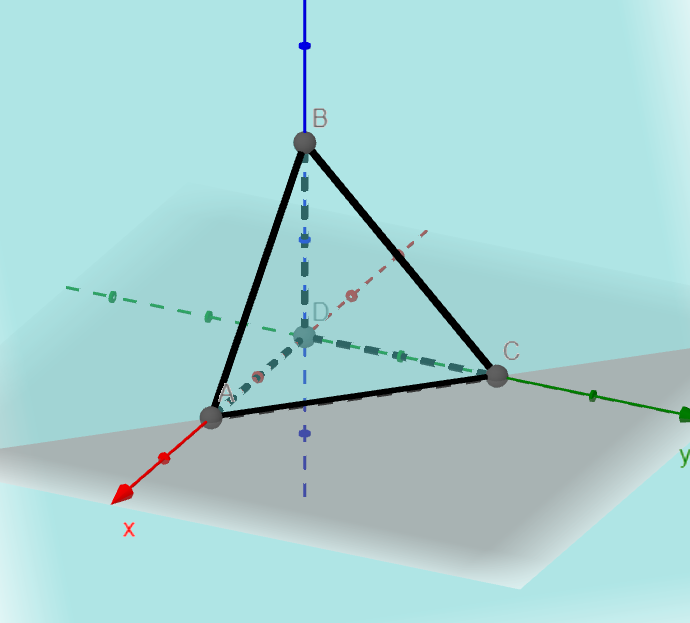
\includegraphics[height=7cm]{calculus/images/calculus_2024_02_14_2}

    $S(x) = S_{DBC} = \frac{(a - x)^2}{2}$

    Тогда $V = \int_0^a \frac{1}{2} (a - x)^2 dx = \frac{1}{2} \int_0^a (x - a)^2 dx =
    \frac{1}{2} \int^a_0 (x - a)^2 d(x - a) = \frac{1}{6} (x - a)^3 \Big|^a_0 = \frac{a^3}{6}$

    \Nota \hypertarget{volumeofbodyofrevolution}{Объем тела вращения}

    Пусть дана функция $r(x)$, задающая радиус тела вращения на уровне $x$,
    тогда объем тела вращения будет равен $\int_a^b \pi r^2(x) dx$

    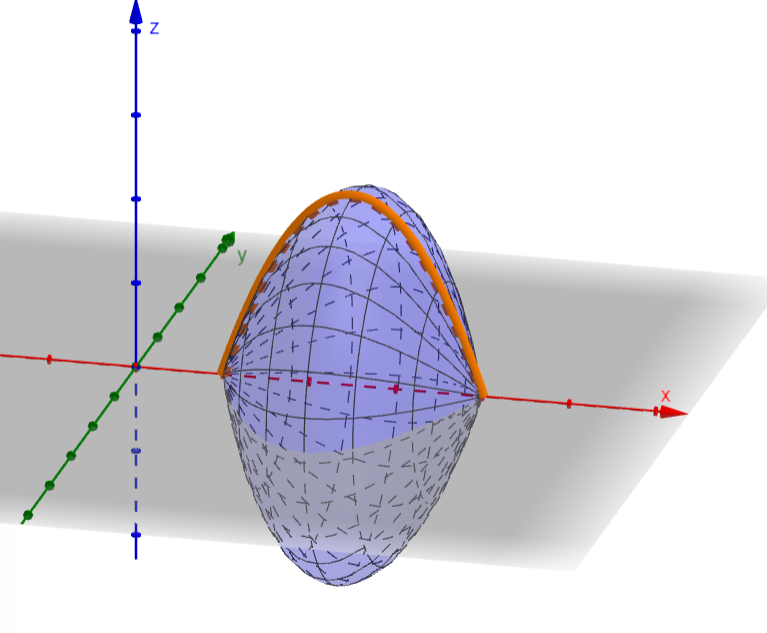
\includegraphics[height=7cm]{calculus/images/calculus_2024_02_14_4}

\end{document}
